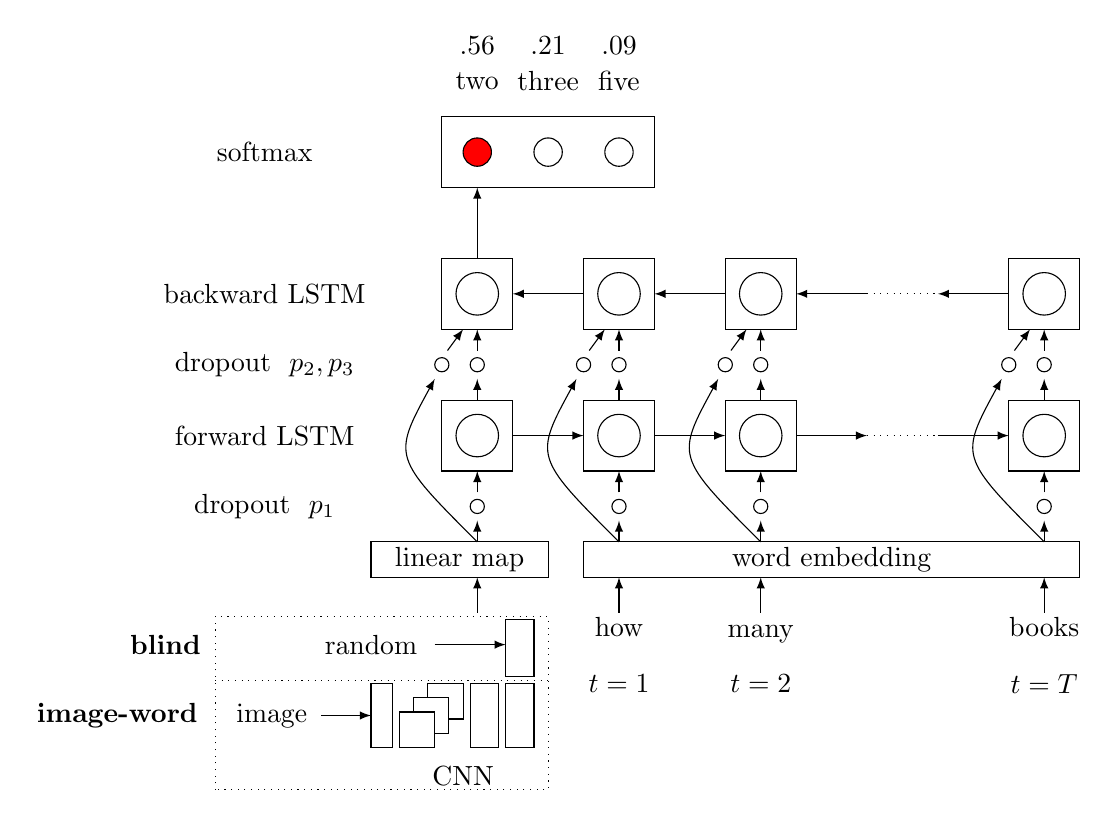
\begin{tikzpicture}[scale=0.9]

\foreach \x in  {5, 7, 9, 13}
{
    \draw (\x,3.0) rectangle (\x+1,4.0);
    \draw (\x+0.5,3.5) circle (0.3cm);
    \draw [-latex](\x+0.5,2.0) -- (\x+0.5,2.3);
    \draw (\x+0.5,2.5) circle (0.1cm);
    \draw (\x-0.0,2.5) circle (0.1cm);
    \draw [-latex](\x+0.5,2.7) -- (\x+0.5,3.0);
}

\foreach \x in  {7, 9, 11, 13}
{
    \draw [latex-](\x-1,3.5) -- (\x,3.5);
}
\draw [dotted] (11,3.5) -- (12,3.5);


\foreach \x in {5.5, 7.5, 9.5, 13.5}
{
    \draw [-latex](\x, 0.0) .. controls (\x-1.2,1.2) .. (\x-0.6,2.3);
    \draw [-latex](\x-0.42, 2.7) -- (\x-0.2, 3.0);
}

\foreach \x in  {5, 7, 9, 13}
{
    \draw (\x,1) rectangle (\x+1,2);
    \draw (\x+0.5,1.5) circle (0.3cm);
    \draw [-latex](\x+0.5,0) -- (\x+0.5,0.3);
    \draw (\x+0.5,0.5) circle (0.1cm);
    \draw [-latex](\x+0.5,0.7) -- (\x+0.5,1);
}

\foreach \x in  {7, 9, 13}
{
    \draw [-latex](\x+0.5,-1) -- (\x+0.5,-0.5);
}

\foreach \x in  {7, 9, 11, 13}
{
    \draw [-latex](\x-1,1.5) -- (\x,1.5);
}

\path (7.5,-2) node[draw=none] (t0) {$t=1$};
\path (9.5,-2) node[draw=none] (t1) {$t=2$};
\path (13.5,-2) node[draw=none] (tT1) {$t=T$};
\draw [dotted] (11,1.5) -- (12,1.5);

\path (7.5,-1.2) node[draw=none] (w1) {how};
\path (9.5,-1.3) node[draw=none] (w2) {many};
\path (13.5,-1.2) node[draw=none] (w3) {books};
\path (2.5,0.5) node[draw=none] (drop) {dropout $~p_1$};
\path (2.5,1.5) node[draw=none] (lstm1) {forward LSTM};
\path (2.5,2.5) node[draw=none] (drop) {dropout $~p_2, p_3$};
\path (2.5,3.5) node[draw=none] (lstm1) {backward LSTM};
\draw (7, -0.5) rectangle (14, 0);

\draw (5,5) rectangle (8,6);
\draw[fill=red] (5.5,5.5) circle (0.2cm);
\draw (6.5,5.5) circle (0.2cm);
\draw (7.5,5.5) circle (0.2cm);
\path (2.5,5.5) node[draw=none] (logit) {softmax};
\path (5.5,6.5) node[draw=none] (logit2) {two};
\path (6.5,6.5) node[draw=none] (logit3) {three};
\path (7.5,6.5) node[draw=none] (logit5) {five};
\path (5.5,7) node[draw=none] (logit2) {.56};
\path (6.5,7) node[draw=none] (logit3) {.21};
\path (7.5,7) node[draw=none] (logit5) {.09};
\draw [-latex] (5.5,4) -- (5.5,5);

\draw (4,-0.5) rectangle (6.5, 0);
\path (5.25,-0.25) node[draw=none] (imgMap) {linear map};

\draw (4.0, -2.9) rectangle (4.3, -2);
\draw[fill=white] (4.8, -2.5) rectangle (5.3, -2);
\draw[fill=white] (4.6, -2.7) rectangle (5.1, -2.2);
\draw[fill=white] (4.4, -2.9) rectangle (4.9, -2.4);
\draw (5.4, -2.9) rectangle (5.8, -2);
\draw (5.9, -2.9) rectangle (6.3, -2);
\draw (5.9, -1.9) rectangle (6.3, -1.1);
\draw [-latex] (5.5, -1.0) -- (5.5, -0.5);

\draw [-latex] (4.9,-1.45) -- (5.9, -1.45);
\draw [-latex] (3.3,-2.45) -- (4.0, -2.45);
\path (4.0,-1.45) node[draw=none] (random) {random};
\path (2.6,-2.45) node[draw=none] (image) {image};
\path (1.1,-1.45) node[draw=none] (blind) {\textbf{blind}};
\path (0.42,-2.45) node[draw=none] (image-word) {\textbf{image-word}};
\path (5.3,-3.3) node[draw=none] (cnn) {CNN};
\draw [dotted] (1.8,-1.95) -- (6.5, -1.95);
\draw [dotted] (1.8,-3.5) rectangle (6.5, -1.05);

\path (10.5,-0.25) node[draw=none] (Wemb) {word embedding};


\end{tikzpicture}